\documentclass[11pt,a4paper]{article}
\usepackage[margin=22mm]{geometry}
\usepackage{amsmath,booktabs,graphicx,siunitx,hyperref}
\title{NAUSICA: 4 mm pitch and 40 ms buckets}
\author{Circuit exercise}\date{\today}
\begin{document}\maketitle
The 4 mm pitch case assumes a mean of 400 ions per pad per 40 ms bucket,
provided by J. J. G\'omez-Cadenas as a design input. The comparison uses the
updated mean of 120 ions for 2 mm pitch and 20 ms buckets.

\section{Circuit and input}
The exercise retains the paper's 180 nm transistor circuit, 1.8 V supply,
20 degree Celsius temperature, external capacitance 1.25 pF and feedback
capacitance 3 fF. The collecting pad remains a 0.5 mm square. M3 has
$W=200\,\mu$m and $L=2\,\mu$m; M4 has $W=2.88\,\mu$m and $L=1.44\,\mu$m.
The archived gate settings and complete model card are recorded in the netlists.
Thermal and flicker noise are evaluated at the DC operating point.

The input uses uniform mean collection times over 40 ms. Each ion follows a
central straight trajectory at 3 m/s through the final 5 mm gap above the pad.
The weighting problem has unit potential on the pad, zero on the surrounding
infinite grounded plane and at infinity, in a homogeneous gas half-space.
The integrated signal is $e[1-\phi_w(g)]$, retained without renormalization.
The 4 mm pitch affects the specified charge population and spatial sampling;
the calculation retains the same local pad benchmark and circuit capacitance.
An electrostatic focusing calculation and event redistribution are separate
inputs to this circuit exercise.

For the 400-ion packet the integrated input charge is 0.06399 fC and the
peak current is 1.5996 fA. Collection begins at simulation time 2 ms and
ends at 42 ms; induction starts before collection.

\section{Readout and results}
At frame boundaries the voltage is averaged over centred 300 $\mu$s windows.
After subtraction of a matched zero-input baseline, the measured difference is
\[
D_n=-[\overline V_n-\alpha\overline V_{n-1}],\qquad
\alpha=e^{-\Delta t/\tau_0}.
\]
The decay time is fitted from the 100-ion packet between 41 and 120 ms after
first collection. The output-noise spectrum is the same as the paper's circuit;
its filtered integral is recalculated for the 40 ms separation:
\[
\sigma_D^2=\int_{0.1\,\mathrm{Hz}}^{1\,\mathrm{MHz}}S_V(f)
\left|\frac{\sin(\pi fT_a)}{\pi fT_a}\right|^2
\left|1-\alpha e^{-2\pi i f\Delta t}\right|^2\,df.
\]
The small-signal ENC is $\sigma_D/g$. The 400-ion signal and S/N are obtained
from a finite-charge SPICE transient. The 20 ms mean signal uses the saved
small-signal calibration multiplied by 120.

\begin{center}\begin{tabular}{lrr}\toprule
Quantity & 2 mm / 20 ms & 4 mm / 40 ms\\\midrule
Mean ions per bucket & 120 & 400 \\
Gain ($\mu$V/ion) & 27.119 & 27.089 \\
Readout noise (mV RMS) & 3.056 & 3.772 \\
ENC ($e$ RMS) & 112.70 & 139.25 \\
Mean signal (mV) & 3.254 & 10.831 \\
Mean signal-to-noise ratio & 1.065 & 2.871 \\
Fitted discharge time (s) & 2.45416 & 2.45416 \\
\bottomrule\end{tabular}\end{center}
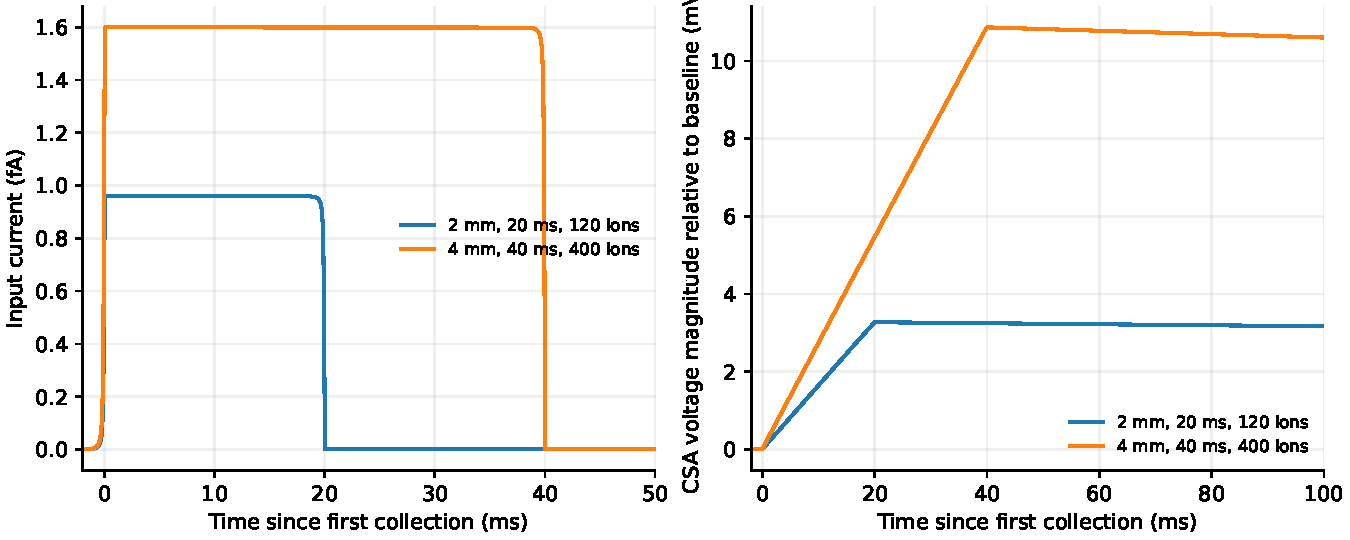
\includegraphics[width=\linewidth]{response_comparison.pdf}

The following populations correspond to illustrative S/N values in the linear
model. Reconstruction can combine information from neighbouring measurements;
these values specify individual-bucket significance.
\begin{center}\begin{tabular}{rr}\toprule
S/N & Ions per 40 ms bucket\\\midrule
1 & 139.2 \\
2 & 278.5 \\
3 & 417.7 \\
5 & 696.2 \\
\bottomrule\end{tabular}\end{center}
The nominal spatial sampling changes from 2 to 4 mm transversely and from 2 to
4 mm along drift, using 0.1 m/s bulk ion speed. The assumed mean population
must be evaluated together with track and blob preservation at that sampling.

\section{Noise contributions and validation}
\begin{center}\begin{tabular}{lr}\toprule
Device & Fraction of filtered noise variance (\%)\\\midrule
V(m1) & 1.3 \\
V(m2) & 12.8 \\
V(m3) & 3.2 \\
V(m4) & 17.8 \\
V(m5) & 0.0 \\
V(m6) & 1.3 \\
V(mf) & 63.6 \\
\bottomrule\end{tabular}\end{center}
The calculation compares 5 and 2.5 $\mu$s transient steps, 200 and 400 frequency
points per decade, and quadrature orders 8 and 16. It checks charge conservation,
independent analytical-current quadrature, 10- and 100-ion discharge fits,
local fit windows, and linearity through 400 ions. Twenty saved-result checks pass.
\begin{center}\begin{tabular}{lr}\toprule
Check & Relative error\\\midrule
transient error & 2.01e-05 \\
spectral error & 6.36e-07 \\
quadrature error & 9.13e-14 \\
tail fit relative error & 2.5e-08 \\
tau timestep error & 5.08e-06 \\
noise variance closure error & 4.15e-07 \\
\bottomrule\end{tabular}\end{center}

\section{Reproduction}
From the repository root, with the pinned Python and Julia dependencies:
\begin{verbatim}
PYTHONPATH=src python scripts/run_pitch_exercise.py \
  --julia /path/to/julia --simulator /path/to/LTspice
\end{verbatim}
Julia performs the input calculation, reduction and checks. HDF5 stores inputs,
raw transients, the reused noise spectrum, numerical results and provenance.
Python acquires LTspice output and generates this report and figure. Presentation
alone is regenerated with \texttt{python scripts/present\_pitch\_exercise.py}.
\end{document}
